\section{Operational architecture}
\label{sec:architecture}


\subsection{Process, feedback, and perspectival description}

The architecture is intentionally process-based. Whitehead's process philosophy is a historical precedent for treating events, transitions, and relations as primary descriptive units rather than reducing the analysis to static substances \parencite{Whitehead1978}. Wiener's cybernetics supplies the explicit language of feedback, communication, and control \parencite{Wiener1948}. Von Neumann's analyses of measurement and self-reproducing automata show why an observer, apparatus, description, and update rule cannot always be treated as independent endpoints \parencite{VonNeumann1955,VonNeumann1966}. Leibnizian perspectivism provides an earlier comparison for the idea that one world may admit multiple internally coherent representations \parencite{Leibniz1989}. None of these sources is identical to the map developed below. They explain why the complete object is a recursive transformation system rather than a single passive observation.

Bohm's distinction between implicate and explicate order and the Bohm--Hiley account of undivided quantum process are retained as comparative physical programs, not as assumptions of the present analysis \parencite{Bohm1980,BohmHiley1993}. The present theory requires only declared maps and equivalence relations. It does not infer an implicate order, a quantum ontology, or a universal process metaphysics from noninjectivity.

\subsection{The complete recursive scientific cycle}

The formal theory is a local core inside a larger scientific cycle. Let \(S(t)\) denote a physical or modeled state at time \(t\). Let \(A_i\) denote an apparatus, intervention, or sampling procedure. Let \(E_i\) denote a finite encoding or reconstruction step. Let \(O_i\) denote the representation accessible to an observer. Let \(L_i\) denote a reportable model, estimate, or claim. Let \(P_i\) denote a prediction, intervention, or next experimental choice. One cycle has the form
\[
S(t)
\longrightarrow A_i
\longrightarrow E_i
\longrightarrow O_i
\longrightarrow L_i
\longrightarrow P_i
\longrightarrow S(t+\Delta t).
\]
The final state enters the next cycle through new measurement. The complete process is recursive. This perception-action-return structure is compatible with predictive-processing and active-inference accounts in which observations update a generative model and actions change subsequent observations \parencite{RaoBallard1999,Friston2010,Parr2022,Friston2025ScaleFree}.

\begin{figure}[tbp]
\centering
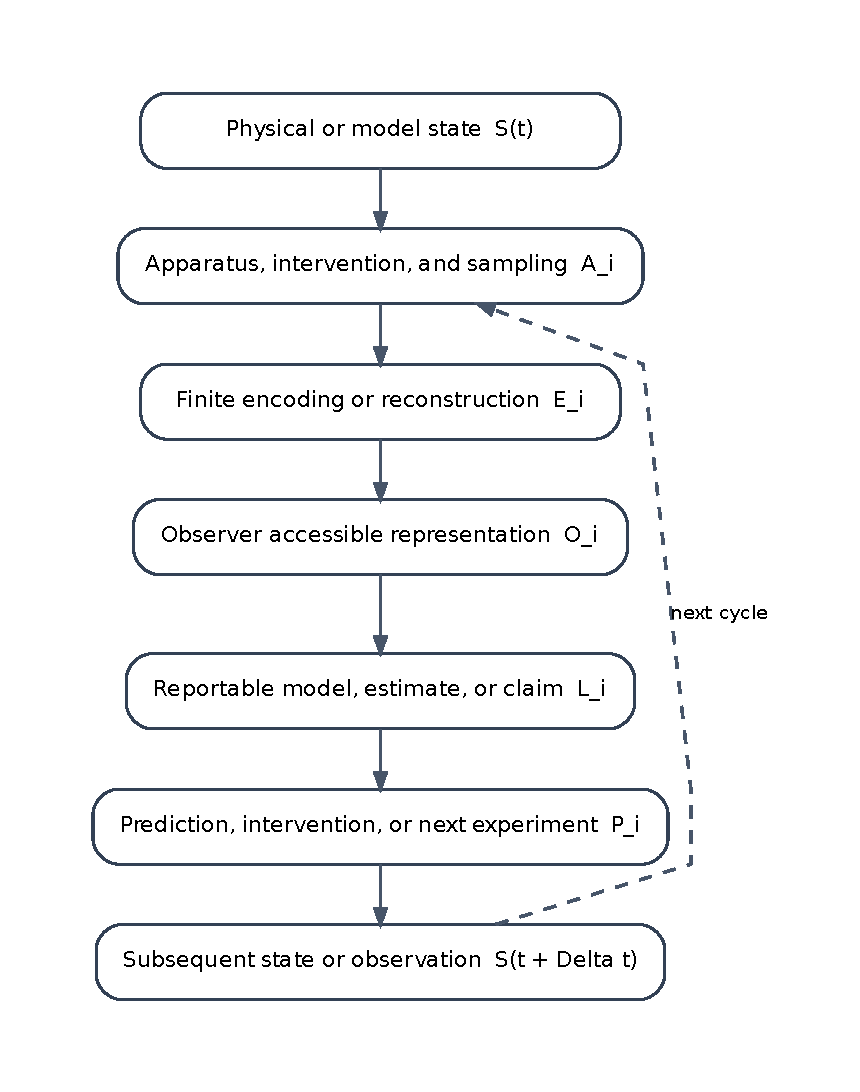
\includegraphics[height=0.67\textheight]{figures/concept_recursive_architecture.pdf}
\caption{Top-down scientific architecture. The map studied in this paper is the reduced local core of a longer recursive cycle. The dashed return marks prediction, intervention, and subsequent observation. The diagram is conceptual rather than a simulation output.}
\label{fig:recursivearchitecture}
\end{figure}

A physical state is not identical to an apparatus output. An apparatus output is not identical to a reconstructed feature. A reconstructed feature is not identical to an internal representation or report. A report is not identical to the next state of the system. Each arrow requires an explicit map.

\subsection{A distributed family of boundaries}

The complete route is better represented as a composition:
\[
X_{\mathrm{phys}}
\xrightarrow{\pi_{\mathrm{app}}}
O_{\mathrm{app}}
\xrightarrow{\pi_{\mathrm{bio}}}
O_{\mathrm{bio}}
\xrightarrow{\pi_{\mathrm{rep}}}
O_{\mathrm{rep}}
\xrightarrow{e}
R
\xrightarrow{a}
X'_{\mathrm{phys}}.
\]
The maps may correspond to physical coupling, detector response, sampling, reconstruction, biological sensing, attention, memory, language, or experimental decision. The aggregate observation map is
\[
\pi=\pi_{\mathrm{rep}}\circ\pi_{\mathrm{bio}}\circ\pi_{\mathrm{app}}.
\]
If two distinct original source states reach the same intermediate value, every subsequent deterministic map preserves that equality. The composite is then noninjective. Noninjectivity of a stage outside the range reached by preceding stages is insufficient; a counterexample is given in \Cref{app:scopechecks}. Refining a later report cannot recover a distinction that was already collapsed upstream unless new information enters through another route.

The stages should eventually be modeled separately rather than compressed into one aggregate map. Apparatus response, sampling, biological transduction, internal representation, report, and action may each preserve different relations and collapse different distinctions. Stage-specific models would show where a loss first occurs and whether later measurements introduce genuinely new information or only re-encode what has already passed through an earlier boundary.


\subsection{Computation as an interface-bound physical process}

A computation implemented in the world is not identical to its abstract description. It requires a physical encoding, a physical evolution, and a readout:
\[
S_{\mathrm{phys}}
\xrightarrow{\eta}
C
\xrightarrow{U}
C'
\xrightarrow{\rho}
R.
\]
Here \(\eta\) assigns an abstract computational state to a physical condition, \(U\) is the declared abstract evolution, and \(\rho\) converts a final physical or encoded state into a reportable result. Frameworks for physical computation make this representation relation explicit and distinguish the abstract calculation from the device that realizes it \parencite{Horsman2014,Horsman2015}. When the computation is embedded inside the system being studied, both \(\eta\) and \(\rho\) are themselves observer interfaces.

The distinction matters because different physical computers do not expose the same state space, elementary operations, error model, or readout. A digital computer represents finite symbolic states through engineered voltage ranges. An analog computer uses calibrated continuous physical variables to approximate a differential relation \parencite{Shannon1941}. A quantum computer manipulates quantum states but ultimately requires a controlled physical implementation and a classical measurement interface \parencite{DiVincenzo2000,AharonovCotlerQi2022}. A brain--computer interface converts selected electrophysiological activity into device commands and requires adaptation of both the user and decoder \parencite{Wolpaw2002,Willett2023}. Human reasoning is mediated by sensory transduction, neural dynamics, memory, language, and report. Equality of an output across these systems does not imply equality of their internal logic, physical representation, or relation to the world.

\begin{table}[tbp]
\centering
\caption{Examples of physically distinct interfaces. The rows are not claimed to be mathematically equivalent. They show why a result must be interpreted relative to the encoding, accessible state, readout, and failure conditions of the particular interface.}
\label{tab:heterogeneousinterfaces}
\small
\begin{tabularx}{\textwidth}{@{}p{0.19\textwidth}p{0.31\textwidth}X@{}}
\toprule
Interface & Accessible state and readout & Principal boundary \\
\midrule
Digital computer & Finite symbolic words encoded by engineered voltage ranges and returned through a discrete output channel. & Word length, architecture, numerical precision, software semantics, and the mapping between physical voltage and symbol. \\
Analog computer & Continuous voltages, currents, rotations, or other calibrated quantities interpreted as variables in a differential model. & Noise, drift, dynamic range, calibration, and the approximation relating physical trajectory to mathematical solution. \\
Quantum computer & Prepared quantum states, controlled transformations, and measurement outcomes converted into classical records. & State preparation, decoherence, permitted measurements, sampling, error correction, and the quantum--classical readout boundary. \\
Brain--computer interface & Selected neural signals translated into commands, text, movement, or another device output. & Electrode placement, signal preprocessing, decoder training, adaptation, and the distinction between intended state and decodable signal. \\
Human sensory and cognitive interface & Receptor signals integrated through neural dynamics, memory, attention, language, and report. & Biological bandwidth, selective attention, prior structure, state dependence, and reportability. \\
Multisensor suite and fused state estimate & Heterogeneous measurements combined with a dynamical model or reference data into an estimated state, residual, confidence value, or track. & Coverage, calibration, synchronization, bias, correlated error, fusion rule, model mismatch, and unobserved state components. \\
Inertial guidance and state estimation & Accelerometer and gyroscope signals combined with a dynamical model to maintain an estimated position, velocity, attitude, and error state. & Sensor bias, drift, model mismatch, initialization, reference updates, and uncertainty in the estimated state. \\
Particle detector and analysis pipeline & Detector interactions reconstructed into tracks, energies, event classes, likelihoods, and parameter limits. & Acceptance, efficiency, resolution, trigger selection, reconstruction assumptions, background model, and statistical decision rule. \\
\bottomrule
\end{tabularx}
\end{table}

A sensor suite gives a concrete example of a distributed boundary. No individual sensor measures the complete state of a vehicle or environment. Each channel returns a partial representation with its own bandwidth, geometry, calibration, noise, and blind regions. Multisensor fusion combines those reports into an estimated state or decision, but the fusion process does not remove the interface. The result remains conditional on sensor coverage, synchronization, uncertainty models, and the rule used to combine observations \parencite{HallLlinas1997,DurrantWhyteHenderson2008}.

The familiar joke that a missile ``knows where it is because it knows where it is not'' is not a technical account of guidance. Its useful core is the role of discrepancy. A sensor suite used to guide or track a missile, a reentry vehicle carrying a warhead, or a spacecraft compares an evolving state estimate with incoming measurements and reference constraints. The residual identifies disagreement between prediction and accessible evidence; it does not reveal an unrestricted external ground truth. The system therefore acts from a bounded coordinate model and quantified uncertainty rather than direct possession of its complete physical state \parencite{Kalman1963,HallLlinas1997,TittertonWeston2004}. This is an interface example, not an operational description of weapon design or use.

Particle physics also requires several meanings of a ``forbidden zone'' to be kept separate. A region may be kinematically forbidden by a specified theory, outside detector acceptance, unobservable because of a blind or dead region, or statistically excluded by data under a model and confidence procedure. Experimental exclusion regions are therefore conditional on the detector, event reconstruction, background model, parameterization, and statistical rule \parencite{Cowan2011,ParticleDataGroup2026}. Exclusion is a strong scientific result, but it is not the same statement as absolute nonexistence independent of the declared interface and model.

Formal exactness and physical approximation must likewise be separated. A proof can be exact relative to its encoded definitions and inference rules, while every physical implementation of the proof checker, sensor, or simulation remains dependent on finite hardware, representation, and readout. Mechanical verification establishes that the encoded conclusion follows from the encoded premises. It does not establish that the encoding is the only possible formalization of human reasoning or that a formal state is identical to the brain's reality interface.

\subsection{Preservation, transformation, compression, dispersion, and collapse}

The phrase \emph{information loss} does not identify what a map has done. The following taxonomy is used throughout the interpretation and future-work sections.

\begin{table}[tbp]
\centering
\caption{Taxonomy of outcomes across an observation or representation map.}
\begin{tabularx}{\textwidth}{@{}p{0.19\textwidth}X X@{}}
\toprule
Outcome & Structural meaning & Mathematical or empirical question \\
\midrule
Preservation & A relation, value, or invariant survives the map. & Which quantities factor through the interface, and are they complete for the target task? \\
Re-encoding & Structure is expressed in a different representation. & Is the transformation invertible, approximately invertible, or only relation-preserving? \\
Compression & The accessible representation contains fewer distinguishable classes than the source. & Which fibers are enlarged, and what refinement would split them? \\
Dispersion & Correlations or organized structure spread across degrees of freedom, time, or scale. & Which observables still carry the relation, and at what scale or resolution? \\
Collapse & Distinct source states map to one accessible state. & Is the map noninjective, and what latent properties vary inside a fiber? \\
Inaccessibility & A structure may remain in the source but lies outside the declared observation channel or threshold. & Does another interface represent it, or is its existence itself underdetermined? \\
Physical destruction & The source structure no longer exists under a domain-specific criterion. & What physical law, measurement, or dynamical model establishes destruction rather than nonrepresentation? \\
\bottomrule
\end{tabularx}
\label{tab:mappingtaxonomy}
\end{table}

A relation can be preserved while its carrier changes. A signal can be transformed without being destroyed. A source distinction can be real but inaccessible to one interface. Conversely, a mathematically possible hidden distinction need not be physically real. The taxonomy prevents \emph{unobserved}, \emph{compressed}, \emph{dispersed}, and \emph{destroyed} from being used as synonyms.

\subsection{External analyst and embedded observer}

Two observational positions must be distinguished. An external analyst can define a model, inspect its source space, and compare it with the observation map. An embedded observer is itself represented within the physical and informational process it is attempting to model. Its self-model, measurement tools, and inference rules are generated and updated within the same larger dynamics.

The present formalization uses the external analyst's mathematical viewpoint to prove facts about a declared interface. It does not yet formalize a system whose model of itself modifies the system that performs the modeling. That embedded problem is closer to second-order cybernetics, autopoiesis, active inference, and recent work on self-referential living systems \parencite{VonFoerster1981,MaturanaVarela1980,Friston2010,Abramsky2025}. It is identified in \cref{sec:limitations} as the next major formal extension.

\subsection{Reduction to the formal core}

The current theorem sequence isolates
\[
X\xrightarrow{\pi}O\xrightarrow{e}R,
\]
where \(X\) is the source or latent state space, \(O\) is the accessible observation space, and \(e:O\to R\) is an admissible experiment. The reduced map may represent one boundary or the composition of many. It is not a replacement for the complete cycle. It is the smallest local object on which the reconstruction question can be stated and proved.

\subsection{Three levels of description}

The mathematical core keeps three object levels separate. A \emph{source state} is an element of \(X\). An \emph{accessible observation} is an element of \(O\). An \emph{experimental result} is an element of \(R\). Two source states can produce one observation. Two models can produce one reachable observation set. Several observations can produce one result. Each equality is relative to the map that defines it.

\subsection{Local noninvertibility}

For \(o\in O\), the fiber is
\[
\pi^{-1}(o)=\{x\in X:\pi(x)=o\}.
\]
When this set contains multiple states, the observation identifies the fiber but not a unique member.

\begin{figure}[tbp]
\centering
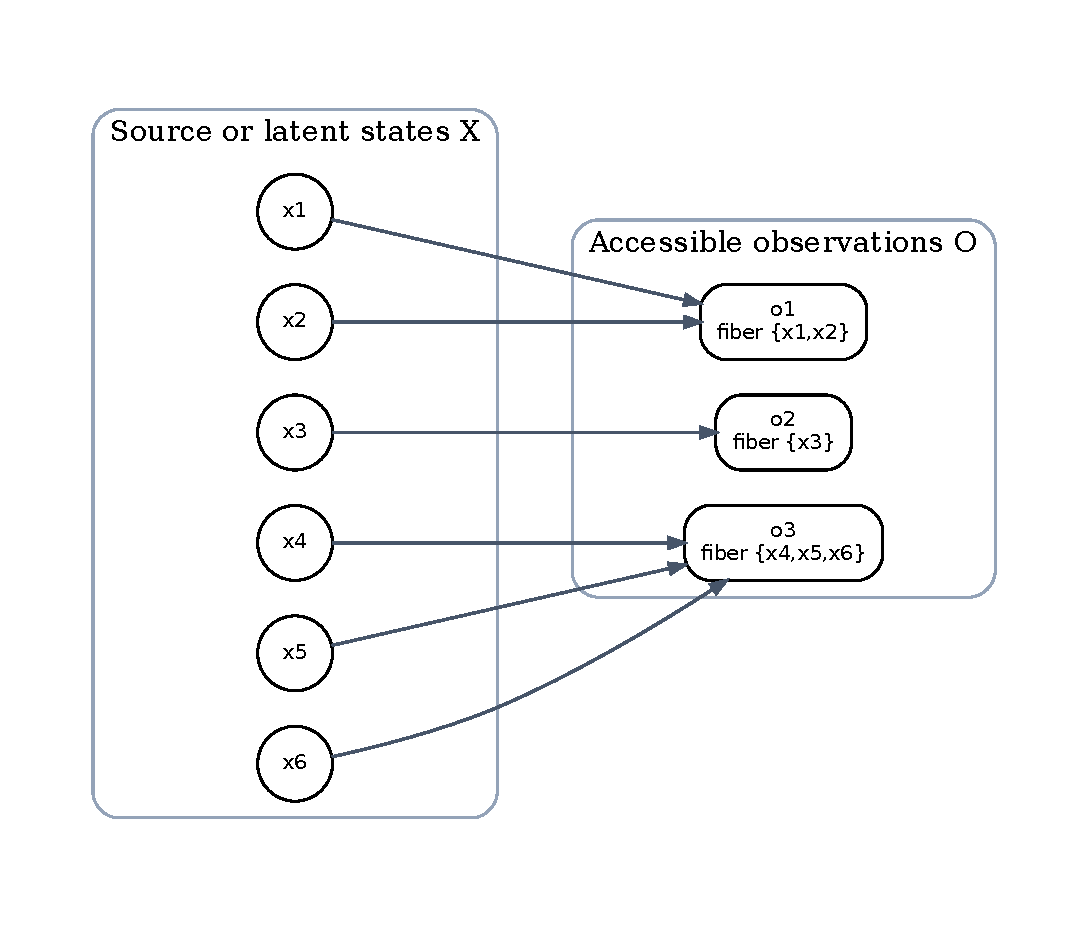
\includegraphics[width=0.82\textwidth]{figures/concept_observation_fibers.pdf}
\caption{Observation fibers. States in one fiber produce the same accessible value. Fiber membership is relative to the specified map. A refined interface may split a fiber that a coarse interface leaves merged.}
\label{fig:observationfibers}
\end{figure}

The accessible value contains no internal tag selecting its source member. A reconstruction claim must therefore use an injective interface, an independently justified restriction on the source class, or additional information supplied from outside the current observation value.
